\newpage
\section{Report 05: POPs treatment of the $Ras^{v12/Ig}$ model (Toxaphene)}

\subsection*{2021-05-13}

\subsection{Introduction}

With the $Eyeful$ model built in last experiment, we are now able to use different kind of POPs to treat the model flies and collect relevant data about the impact of POPs on \textbf{tumor migration}.

Other phenotypes, such as the \textbf{adult survival rate}, \textbf{reproductive capacity} and \textbf{body weight} will also be measured, if possible. These data can be used to study the overall effects of POPs, and they can provide clues about the factors behind tumor migration.

\subsection{Experiment Design}

\subsubsection{POPs gradients}
The setting of the POPs gradients used in the experiments is of much importance for their implementation.
For the convenience of calculation and dilution, we choose \textbf{Mass fraction} ($m_{POPs}/m_{fly food}$) as the unit of concentration.
According to previous literature and the real situation of the POPs pollution, we choose several POPs, which are listed in the table below. Considering that solvent should not pose much impact to our model, we choose \textbf{Dimethyl Sulfoxide (DMSO)} as the solvent for the hydrophobic POPs (in this experiment, Chlordecone). The POPs is dissolved in DMSO, and the added directly in to fly food.
As to the concentration of POPs, we started at $10^{-4}$ and dilute 10x to $10^{-6}$ to make a gradient of three concentrations, according to previous report of the POPs pollution.


\subsubsection{Crossing scheme}
The $Ras^{v12/Ig}$ model consists of two lines:
\begin{enumerate}
    \item w;$Igl^4$ FRT40A UAS-$RAS^{v12}$/CyO;Sb/TM6B Tb
    \item yw ey-Flp; tub-Gal80 FRT40A; act>y+>Gal4 UAS-GFP
\end{enumerate}
The Crossing scheme is shown below.
\begin{enumerate}
    \item \female w;$Igl^4$ FRT40A UAS-$RAS^{v12}$/CyO;Sb/TM6B Tb $\times$ yw ey-Flp; tub-Gal80 FRT40A; act>y+>Gal4 UAS-$GFP$ \male
    \item \female yw ey-Flp; tub-Gal80 FRT40A; act>y+>Gal4 UAS-GFP $\times$ w;$Igl^4$ FRT40A UAS-$RAS^{v12}$/CyO;Sb/TM6B Tb \male
\end{enumerate}

\subsubsection{Measurements}
After the crossing is done, we did several measurements everyday at the same time.

\begin{enumerate}
    \item Number of adults alive in the tube (optional) 
    \item Number of egg laid (optional)
    \item Number of adults with \textbf{tumor migration}
\end{enumerate}
After each day, transfer the adults to a new tube.

\subsection{Materials \& Methods}

\subsubsection{Preparation of fly food with POPs gradients}
The steps is listed below.
\begin{enumerate}
    \item Add \SI{1000}{\micro\liter} Dimethyl Sulfoxide (DMSO) to the POPs, lable as \texttt{\#stock solution}.
    \item Vortex till the POPs is completely dissolved.
    \item Calculate the concentration of the \texttt{\#stock solution}.
    \item Dilute the \texttt{\#stock solution} to fly food to make the gradients.
    \item Pour the fly food to tubes.
\end{enumerate}

\subsubsection{Crossing of the flies}

\paragraph{Virgins}
To carry out crosses cleanly, you must start with virgin females. Female flies are capable of mating as early as possible after emerging from the pupae stage and are polyandrous(capable of mating with several males). Once mated Females can retain viable sperm for several days and this will confuse the results of a subsequent controlled mating. Therefore, it is necessary to collect enough virgins before we carry out the crossing.

\paragraph{Crossing}
In the crossing, we used the tools needed for basic fly experiments mentioned in Lab Report 04.
	
Here are the steps:
	
		\begin{enumerate}
			\item Empty the stocks before collecting the virgins.
			\item Collect the virgins for several mornings, make sure the virgins have the required phenotypes.
			\item Anesthetize the flies before making the crossing to check the phenotypes. Then put the virgins with the corresponding males in a tube. Record and mark the genotype and numbers of the files.
			\item Put the crossings in \SI{25}{\celsius} with  60-65\% relative humidity. Wait for about a week for the crossings to give the F1 flies.
			\item Collect the F1 larva of the 3rd instar with the desired phenotype.
		\end{enumerate}

\subsubsection{Record of the results}
Different from the $Eyeful$ model, the $Ras^{V12}$ model can not survive to adults, and therefore dissection is needed in order to observe tumours and metastases. The eye disc, brain and ventral nerve cord are what we need from dissection.

The equipment needed for dissection is listed below.

\begin{itemize}
    \item Dissecting microscope
    \item Two pairs of sharp forceps (Dumont, no. 5)
    \item Dissection dishes
    \item Microscope slides
    \item PBST Solution
\end{itemize}

The steps of dissection is listed below, and the protocol is from Joy S Wu \& Liqun Luo.

\begin{enumerate}
    \item Collect larva of the stage of interest.
    \item Place the larvae into a dissection dish containing cold PBST.
    \item Use two forceps to tear the larva into halves.
    \item Overturn the skin of front half of the larva.
    \item Peeling the larval cuticle apart like a banana, starting at the mouth hook. 
    \item Discard the larval body. While maintaining a grip on the mouth hook, gently remove excess tissue surrounding the eye disc, brain and ventral nerve cord.
\end{enumerate}

The eye disc, brain and ventral nerve can then be observed using a Fluorescence Microscopy.

Videos that shows how dissection works can be found on \url{https://www.janelia.org/project-team/flylight/protocols}.
\subsection{Results \& Discussion}

\subsubsection{A typical result of tumour metastases in this model}
A typical result of tumour metastases from eye disc to brain is shown below. The migrated cells are labeled with GFP.
\begin{figure}[H]
    \centering
    \includegraphics[width=0.5\textwidth,angle=0]{image/VNC.png}
    \caption{A typical result of tumour metastases}
    \label{Eyef}
\end{figure}

\subsubsection{Eye tumour metastases ratio}
The ratio of tumour metastases is shown in the figure below.

\begin{figure}[H]
    \centering
    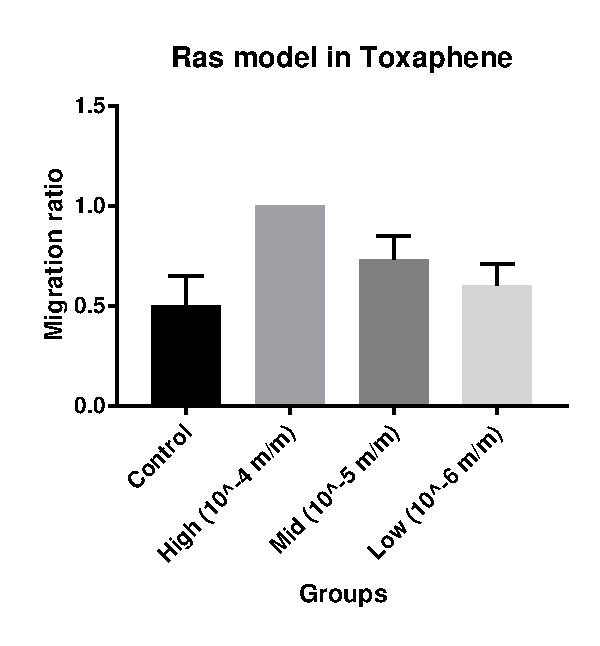
\includegraphics[width=0.6\textwidth,angle=0]{image/Data2.eps}
    \caption{The ratio of tumour metastases}
    \label{Eye}
\end{figure}

\subsubsection{Discussion}
Due to the small number of samples (n=12 for control group, n=3 for $10^{-4}$ group, n=15 for $10^{-5}$ group, n=20 for $10^{-6}$ group), the t-test did not give out significant results, but the figure suggests a tendency that higher concentration of Toxaphene is related to more tumour metastases.

We also noticed that the survival of F1 larva is affected by Toxaphene. Higher level of Toxaphene is not favourable for the survival of F1 larva, and this may cause undesirable impact on the collection of data.